Графиком функции такого вида является половинка параболы

(!) Все обратные функции - это поворот вправо на 90 градусов, а так как в действительных числах не существует корня из отрицательного числа - нижняя ветвь параболы отсутствует. Ну и так же, если бы было две ветви - это противоречило бы определению функции - одному x должен соответствовать 1 y.

\begin{figure}[h!]
	\centering
	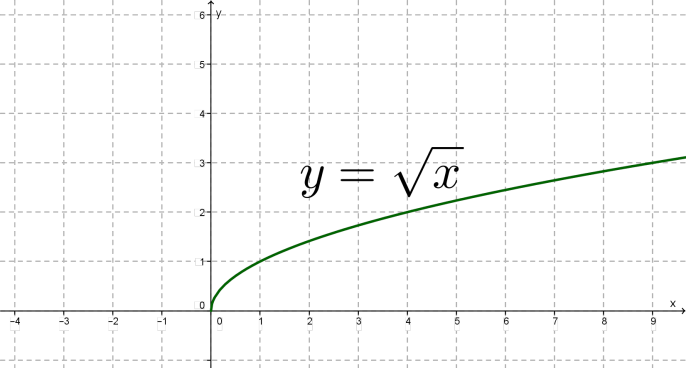
\includegraphics[width=0.5\textwidth]{img/sqrt.png}
	\caption{Функция корня}
\end{figure}

Построение также как и для параболы запоминаем (для простого вида!) точки 1-1 2-4

По точкам, желательно выбирать - 3-4 различных точки для построения.

